\chapter*{Introduction}
\label{cap:introduction}
\addcontentsline{toc}{chapter}{Introduction}

\chapterquote{People think of education as something that they can finish.}{Isaac Asimov}
\section{¿Qué es APRS?}

APRS or Automatic Packet Reporting System (APRS) is a real-time digital communications system that allows the exchange of information between amateur radio stations.

In general, APRS is used for vehicle tracking, transmission of text messages, dissemination of weather information and communication in emergency situations, although due to the flexibility of the protocol it can be used in any other situation.

\begin{figure}[h!]
	\centering
	
\includegraphics[width=0.2\textwidth]{Imagenes/Chapter_1/APRS_logo.png}
	\caption{APRS logo.}
	\label{fig:aprs-logo}
\end{figure}

\section{Main APRS features}

APRS has several features that make it useful and versatile in the field of amateur radio communication, among which are the following:
\begin{itemize}
	\item \textbf{Working frequency:} APRS operates in the VHF band, specifically on the 144.80 MHz frequency in Europe, although other regions of the world use different frequencies as shown in the figure below. \Cref{fig:freq-map}.
	\item \textbf{Transmission mode:} APRS uses as a transmission mode individual packets that have to follow an established format, which greatly facilitates the adoption and integration of this technology.
	\item \textbf{Aprs retransmission policy:} In the APRS system, a packet of information is transmitted multiple times, gradually decreasing the emission frequency of these transmissions as time progresses. This method aims to maximize the packet reception rate.
\end{itemize}

\begin{figure}
	\centering
	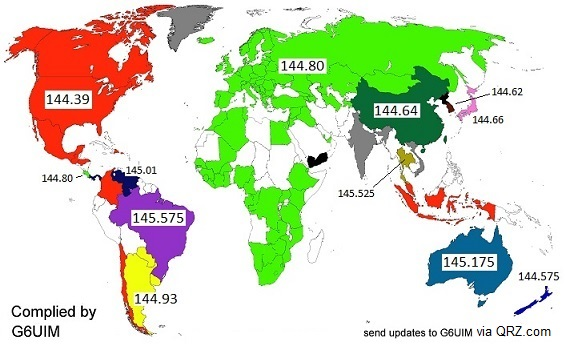
\includegraphics[width=0.5\textwidth]{Imagenes/Chapter_1/mapa_frecuencias_aprs.jpg}
	\caption{Aprs emission frequency around the globe.}
	\label{fig:freq-map}
\end{figure}


\section{Main APRS applications}

\begin{itemize}
	\item \textbf{GPS position reports:} APRS allows users to send their geographic location in the form of coordinates, obtained through GPS systems, which facilitates the tracking of vehicles or people in real time.

	\item \textbf{Weather data:} Weather stations often use APRS messages to report different data such as temperature, humidity or barometric pressure, including updated and useful information for various applications.

	\item \textbf{Internet integration:} Through the APRS-IS system, APRS messages are accessible over the Internet through different nodes, extending the reach and scope of this system.

	\item \textbf{Uso en Emergencias:} In emergency situations, APRS is a vital tool for broadcast communication and tracking of resources and personnel.
\end{itemize}

\section{History and Development of APRS}

The APRS system was born in the 1980s by Bob Bruninga, an engineer working at the U.S. Naval Academy. Bruninga created the first implementation of APRS on an Apple II computer in 1982 for the purpose of mapping Navy position reports on the high seas.\footnote{\url{http://www.aprs.org/APRS-docs/ARTICLES.TXT}}

The first real use of APRS was in 1984, when Bruninga developed a more advanced version on a VIC-20 to report the position and status of horses in an endurance race.

Over the next few years, Bruninga continued to refine the system, which he later dubbed the Connectionless Emergency Traffic System (CETS).

After a series of Federal Emergency Management Agency (FEMA) exercises using CETS, the system was moved to the IGM Pc. During the 1990s, CETS (now known as the Automatic Position Reporting System) continued to evolve.

As GPS technology became more widely available, the term ``Positioning'' was replaced by ``Package'' to better represent the broader capabilities of the system and emphasize its uses beyond mere position reporting.

\begin{figure}[h]
	\centering
	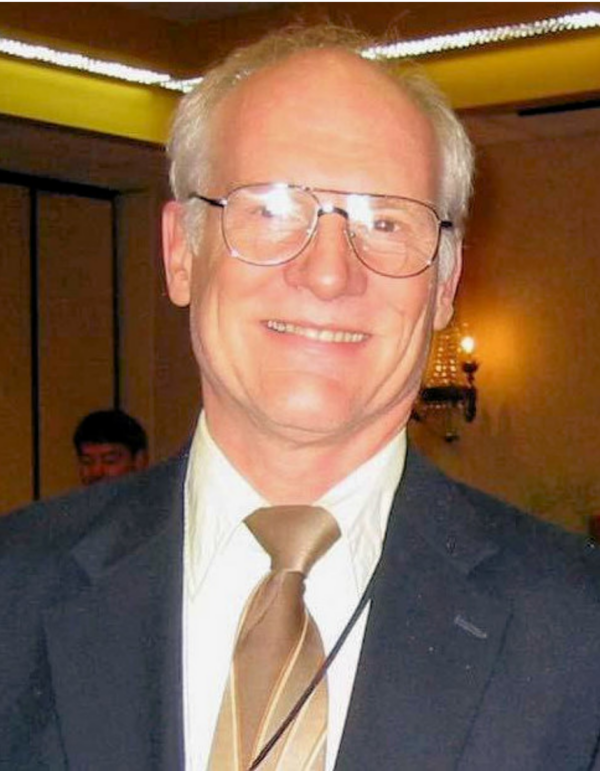
\includegraphics[width=0.15\textwidth]{Imagenes/Chapter_1/bob_bruninga.png}
	\caption{Bob Bruninga (creator of the APRS system).}
	\label{fig:bob-bruninga}
\end{figure}

\section{Work Plan}

For the execution of this project, the following work plan has been proposed, which is divided into the following phases:

\begin{itemize}
	\item \textbf{Phase 1:} Research and Requirements Analysis.
	\item \textbf{Phase 2:} Design and Planning.
	\item \textbf{Phase 3:} Implementation and Development.
	\item \textbf{Phase 4:} Report Writing.
\end{itemize}

Figure \ref{fig:gantt-diagram} shows a Gantt chart with the start and end dates of each of the activities carried out throughout the project.

\begin{figure}[h]
	\centering
	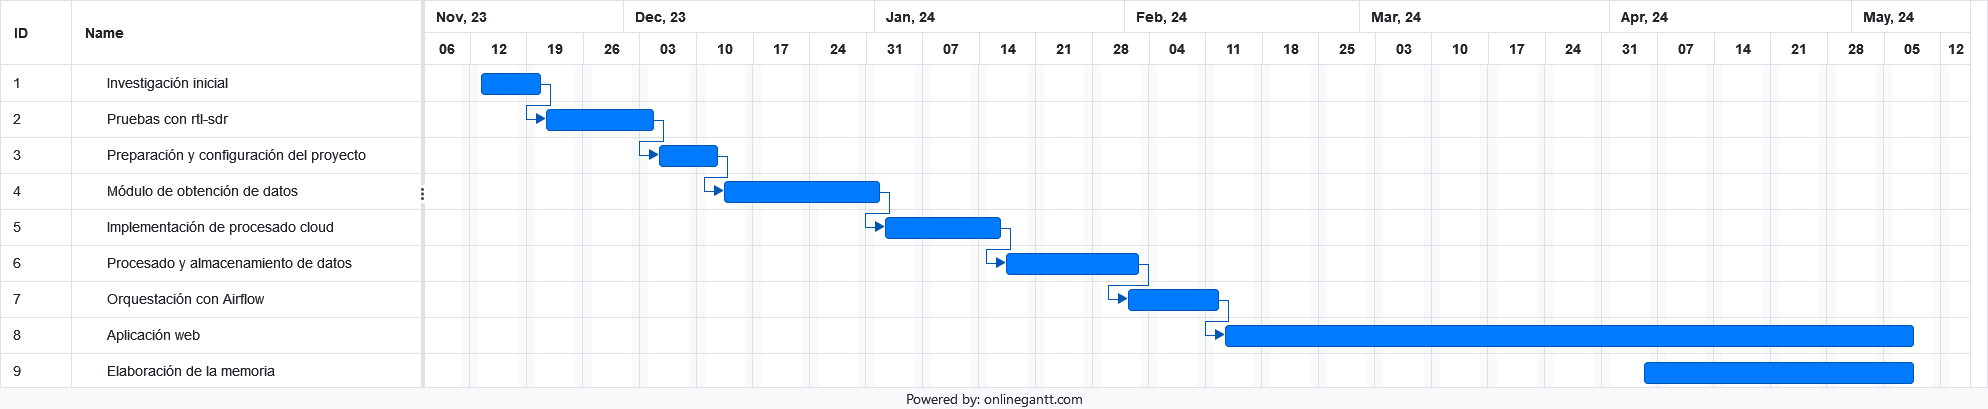
\includegraphics[width=1\textwidth]{Imagenes/Chapter_1/gant.png}
	\caption{Proposed work plan.}
	\label{fig:gantt-diagram}
\end{figure}

Regular meetings have also been held with the TFG supervisors to review progress and discuss any issues encountered during development.

\section{Proposal}
A comprehensive solution is proposed that includes the acquisition, processing, visualization, and analysis of APRS data. The solution will focus on improving the user experience and enriching the available information by integrating data from various open and available sources.

\subsection{Approach}

\begin{itemize}
	\item \textbf{Enhanced User Experience:} The solution will have an intuitive, fast, and useful interface that facilitates navigation and interaction with the data.
	\item \textbf{Advanced Analysis:} The solution will have advanced tools for detailed visualization of APRS traffic, precise filtering, and data analysis, aiming to extract intelligence from received messages.

	\item \textbf{Supplementation:} The solution is not aimed at replacing aprs.fi, aprs.to, or other similar platforms but to offer an alternative with complementary functionalities that enhance the user experience.

	\item \textbf{Information Enrichment:} Data from various open and available sources will be collected to offer a more comprehensive view of APRS traffic and its users, thus improving the quality of information available to users.
\end{itemize}

\subsection{Benefits}

\begin{itemize}
	\item \textbf{Better Understanding of APRS Traffic:} Users will be able to obtain more detailed and actionable information from transmitted messages, allowing them to better understand APRS traffic.

	\item \textbf{More Effective Decision Making:} Integrated data analysis will help users make more informed decisions based on the information received, thereby improving the effectiveness of their actions.

	\item \textbf{Flexibility:} The self-hosting option will allow users to have greater control over their data and privacy, providing greater flexibility in its management.

\end{itemize}

\section{Requirements}

The proposed solution must meet a series of essential requirements to ensure its value and accessibility:

\begin{itemize}
	\item \textbf{Low Cost:} The solution must be economical to ensure accessibility to a wide range of users, including those with limited budgets.

	\item \textbf{Hosting Flexibility:} The solution must offer self-hosting capability; users should be able to choose to host it on their own servers or use the solution in the cloud according to their preferences and specific requirements.

	\item \textbf{Extensibility:} The solution must be extensible, meaning it should allow the integration of new functionalities and expansion of its capacity according to the changing needs of users.

	\item \textbf{Improved Filtering:} More precise and flexible filtering should be provided compared to existing platforms, enabling users to obtain relevant and useful information from APRS data to complement that already provided by alternatives.

	\item \textbf{Integrated Data Analysis:} The solution must include integrated data analysis to help users better understand the information received via APRS and derive valuable insights and conclusions from transmitted messages.

\end{itemize}